\documentclass[border=0pt]{standalone}
\usepackage{amsmath,amssymb}
\usepackage{xcolor}
\usepackage{tikz}
\usetikzlibrary{arrows.meta,calc,decorations.pathreplacing,positioning,shapes.geometric,backgrounds}
\definecolor{c1}{RGB}{0,114,178}
\definecolor{c2}{RGB}{230,159,0}
\definecolor{c3}{RGB}{0,158,115}
\definecolor{cr}{RGB}{213,94,0}
\tikzset{every picture/.append style={show background rectangle,
    background rectangle/.style={fill=white}, inner frame sep=8pt}}
\newcommand{\roll}{\mathcal{R}}
\begin{document}
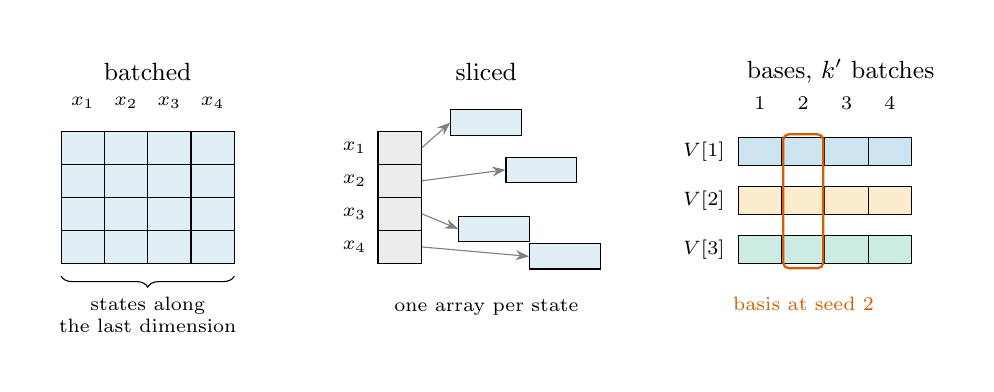
\begin{tikzpicture}[>=Stealth, cell/.style={draw, minimum width=0.55cm, minimum height=0.42cm,
      inner sep=0pt, font=\scriptsize}]
    % ---- batched ----
    \node[font=\small] at (1.1, 2.55) {batched};
    \foreach \j in {1,...,4} {
      \foreach \r in {1,...,4} {
        \node[cell, fill=c1!12] at ({0.55*(\j-1) + 0.275}, {2.0 - 0.42*\r}) {};
      }
      \node[font=\scriptsize] at ({0.55*(\j-1) + 0.275}, 2.15) {$x_\j$};
    }
    \draw[decorate, decoration={brace, mirror, amplitude=4pt}] (0, -0.05) -- (2.2, -0.05)
      node[midway, below=4pt, font=\scriptsize, align=center] {states along\\the last dimension};
    % ---- sliced ----
    \begin{scope}[xshift=4.0cm]
      \node[font=\small] at (1.4, 2.55) {sliced};
      \foreach \j in {1,...,4} {
        \node[cell, fill=gray!15] (p\j) at (0.3, {2.0 - 0.42*\j}) {};
        \node[font=\scriptsize, anchor=east] at (0.0, {2.0 - 0.42*\j}) {$x_\j$};
      }
      \foreach \j/\x/\y in {1/1.4/1.9, 2/2.1/1.3, 3/1.5/0.55, 4/2.4/0.2} {
        \node[cell, fill=c1!12, minimum height=0.32cm, minimum width=0.9cm] (a\j) at (\x, \y) {};
        \draw[->, gray] (p\j.east) -- (a\j.west);
      }
      \node[font=\scriptsize, align=center] at (1.4, -0.45) {one array per state};
    \end{scope}
    % ---- bases ----
    \begin{scope}[xshift=8.6cm]
      \node[font=\small] at (1.3, 2.55) {bases, $k'$ batches};
      \foreach \a/\c in {1/c1, 2/c2, 3/c3} {
        \foreach \j in {1,...,4} {
          \node[cell, fill=\c!20, minimum height=0.36cm] at ({0.55*(\j-1) + 0.275}, {2.15 - 0.62*\a}) {};
        }
        \node[font=\scriptsize, anchor=east] at (-0.05, {2.15 - 0.62*\a}) {$V[\a]$};
      }
      \draw[thick, cr, rounded corners=2pt] (0.55*1 + 0.02, 0.05) rectangle (0.55*2 - 0.02, 1.75);
      \node[font=\scriptsize, cr, align=center] at (0.83, -0.4) {basis at seed 2};
      \foreach \j in {1,...,4} {
        \node[font=\scriptsize] at ({0.55*(\j-1) + 0.275}, 2.15) {$\j$};
      }
    \end{scope}
  \end{tikzpicture}
\end{document}
